\documentclass[11pt]{article}

\usepackage[margin=2.5cm]{geometry}
\usepackage[utf8]{inputenc}
\usepackage[T1]{fontenc}
\usepackage[protrusion=true,expansion=false]{microtype}
\usepackage{float}
\usepackage{booktabs}
\usepackage{graphicx}
\usepackage{caption}
\usepackage{longtable}
\usepackage{array}
\usepackage{siunitx}
\usepackage{xcolor}
\usepackage{fancyhdr}
\usepackage{enumitem}
\PassOptionsToPackage{hyphens}{url}
\usepackage{hyperref}

\hypersetup{
    colorlinks=true,
    linkcolor=blue,
    urlcolor=blue,
    citecolor=blue,
    pdftitle={COVID-19 Vaccination Pace in Brazil, 2021-2022},
    pdfauthor={Prepared with Claude}
}

\sisetup{group-separator={,}, group-minimum-digits=4}

\setlength{\headheight}{14.5pt}
\pagestyle{fancy}
\fancyhf{}
\rhead{COVID-19 Vaccination Pace -- Brazil}
\lhead{2021--2022}
\rfoot{\thepage}

\setlength{\parskip}{0.4em}
\setlength{\parindent}{0pt}
\raggedbottom

\title{\textbf{COVID-19 Vaccination Pace in Brazil (2021--2022)} \\[4pt]
\large Monthly Average Daily Vaccination Rate and Peak Vaccination Days}
\author{Compiled from official Brazilian Ministry of Health data}
\date{\today}

\begin{document}

\maketitle

\begin{abstract}
\noindent This report summarizes the pace of COVID-19 vaccination in Brazil from the start of the
national campaign (17 January 2021) through December 2022. It presents (1) the month-by-month
average number of doses administered per day, with an accompanying chart, and (2) the specific
calendar day on which the highest number of doses was administered in each month. Brazil had no
COVID-19 vaccine in use during 2020; the earliest data available is 17 January 2021, which is why
the analysis begins there rather than in 2020.
\end{abstract}

\section{Data Source and Methodology}
\label{sec:methodology}

The Brazilian Ministry of Health (\emph{Minist\'erio da Sa\'ude}) publishes its official COVID-19
vaccination panel (``Vacina\c{c}\~ao - COVID-19'') as an interactive Power BI-style dashboard hosted at
\url{https://infoms.saude.gov.br}, linked from the department landing page at
\url{https://www.gov.br/saude/pt-br/composicao/seidigi/demas/covid19}. That dashboard is a
JavaScript application with no downloadable data table and is protected against automated access,
so the day-by-day figures behind it cannot be scraped directly.

Instead, this report uses the same underlying official series as compiled, cleaned, and continuously
updated by \textbf{Our World in Data (OWID)}, whose Brazil vaccination time series is sourced directly
from the Brazilian Ministry of Health / OpenDataSUS reporting. This is the standard secondary source
used by researchers and journalists precisely because the primary dashboard is not machine-readable.
Full source details are given in Section~\ref{sec:sources}.

\textbf{Two figures are used from the source data:}
\begin{itemize}[nosep]
    \item \texttt{daily\_vaccinations} -- OWID's smoothed estimate of doses administered per day
    (a 7-day rolling figure, interpolated on days when the government did not publish a daily
    breakdown). This column is used for the \textbf{monthly averages} in Section~\ref{sec:averages},
    since it is essentially complete across the whole period (only the first day of the campaign is
    undefined).
    \item \texttt{daily\_vaccinations\_raw} -- the actual reported day-to-day new-dose count, used to
    identify the \textbf{single calendar day of peak vaccination} in each month (Section~\ref{sec:peaks}).
\end{itemize}

\textbf{Data-quality caveat:} the raw daily breakdown is complete for essentially all of 2021, but
official day-by-day reporting became patchier during 2022 as the campaign wound down -- on some days
only a cumulative running total was published, without a same-day new-dose figure. Coverage (the
share of days in a month with a usable raw value) ranged from 100\% in most of 2021 down to as low as
29\% in some months of 2022. Where coverage is low, the reported ``peak day'' should be read as the
highest \emph{reported} day, not necessarily the true single highest day of the entire month; this is
flagged explicitly in Table~\ref{tab:peaks2022}.

\section{Monthly Average Vaccination Rate per Day}
\label{sec:averages}

Table~\ref{tab:averages} and Figure~\ref{fig:averages} show the average number of doses administered
per day, averaged over each calendar month, from January 2021 (start of the campaign) through
December 2022.

\begin{table}[H]
\centering
\caption{Average doses administered per day, by month (2021--2022)}
\label{tab:averages}
\begin{tabular}{l r @{\hspace{2cm}} l r}
\toprule
\textbf{Month} & \textbf{Avg. doses/day} & \textbf{Month} & \textbf{Avg. doses/day} \\
\midrule
Jan/21\textsuperscript{a} & \num{116305} & Jan/22 & \num{957290} \\
Feb/21 & \num{230500} & Feb/22 & \num{1100371} \\
Mar/21 & \num{407336} & Mar/22 & \num{719655} \\
Apr/21 & \num{785900} & Apr/22 & \num{510743} \\
May/21 & \num{733689} & May/22 & \num{388218} \\
Jun/21 & \num{1017785} & Jun/22 & \num{427119} \\
Jul/21 & \num{1302031} & Jul/22 & \num{402683} \\
Aug/21 & \num{1654413} & Aug/22 & \num{128636} \\
Sep/21 & \num{1511318} & Sep/22 & \num{112450} \\
Oct/21 & \num{1356783} & Oct/22 & \num{11040} \\
Nov/21 & \num{1015730} & Nov/22 & \num{33571} \\
Dec/21 & \num{740331} & Dec/22 & \num{200192} \\
\midrule
\textbf{2021 average} & \textbf{\num{948380}} & \textbf{2022 average} & \textbf{\num{411962}} \\
\bottomrule
\end{tabular}

\vspace{4pt}
\raggedright
{\footnotesize \textsuperscript{a}January 2021 covers only 15 days (17th--31st), since the
campaign started on 17 January 2021.}
\end{table}

\begin{figure}[H]
\centering
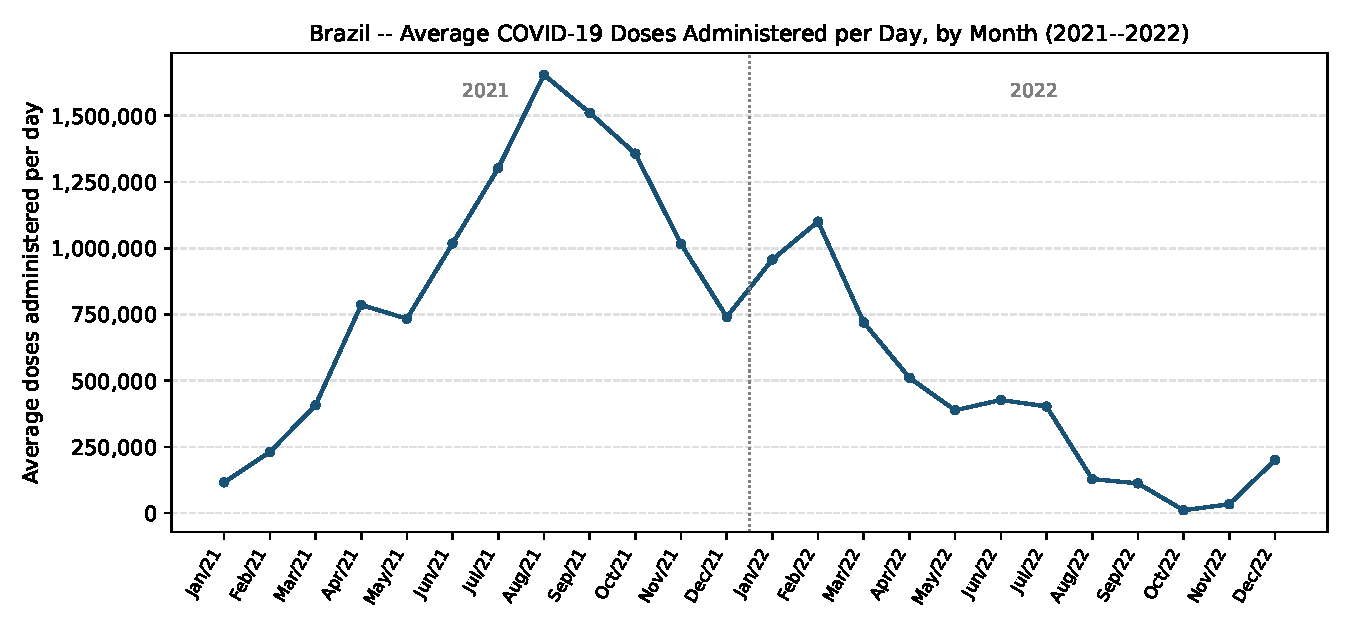
\includegraphics[width=0.95\textwidth]{monthly_avg_doses.pdf}
\caption{Average COVID-19 doses administered per day in Brazil, by month (Jan 2021--Dec 2022).
Source: Brazilian Ministry of Health data, as compiled by Our World in Data.}
\label{fig:averages}
\end{figure}

By the end of 2021, approximately 331 million cumulative doses had been administered nationwide,
at an average pace of about \num{948000} doses per day; by the end of 2022 the cumulative total had
reached approximately 480 million doses, but the 2022 daily average pace had fallen to about
\num{412000} doses per day. The clear peak period of the campaign was August--October 2021, driven
by the mass first- and second-dose rollout; the pace declines steadily through 2022 as most of the
eligible population was already vaccinated and booster uptake slowed.

\section{Day of Peak Vaccination, Month by Month}
\label{sec:peaks}

Tables~\ref{tab:peaks2021} and~\ref{tab:peaks2022} list, for every month from January 2021 to
December 2022, the single calendar day on which the highest number of doses was recorded, together
with that day's dose count and the raw-data coverage for the month (see the caveat in
Section~\ref{sec:methodology}).

\begin{table}[H]
\centering
\caption{Day of peak vaccination per month -- 2021}
\label{tab:peaks2021}
\begin{tabular}{l l r r}
\toprule
\textbf{Month} & \textbf{Peak date} & \textbf{Doses that day} & \textbf{Data coverage} \\
\midrule
Jan/21 & 29 Jan 2021 & \num{360715} & 93.3\% \\
Feb/21 & 12 Feb 2021 & \num{429070} & 100.0\% \\
Mar/21 & 29 Mar 2021 & \num{943825} & 100.0\% \\
Apr/21 & 23 Apr 2021 & \num{1782040} & 100.0\% \\
May/21 & 06 May 2021 & \num{1048363} & 100.0\% \\
Jun/21 & 17 Jun 2021 & \num{2259621} & 100.0\% \\
Jul/21 & 22 Jul 2021 & \num{1932002} & 100.0\% \\
Aug/21 & \textbf{17 Aug 2021} & \textbf{\num{3002675}} & 100.0\% \\
Sep/21 & 10 Sep 2021 & \num{2407953} & 100.0\% \\
Oct/21 & 25 Oct 2021 & \num{2419442} & 100.0\% \\
Nov/21 & 05 Nov 2021 & \num{2022153} & 100.0\% \\
Dec/21 & 03 Dec 2021 & \num{1714641} & 87.1\% \\
\bottomrule
\end{tabular}
\end{table}

\begin{table}[H]
\centering
\caption{Day of peak vaccination per month -- 2022}
\label{tab:peaks2022}
\begin{tabular}{l l r r}
\toprule
\textbf{Month} & \textbf{Peak date} & \textbf{Doses that day} & \textbf{Data coverage} \\
\midrule
Jan/22 & 17 Jan 2022 & \num{3976605} & 87.1\% \\
Feb/22 & 18 Feb 2022 & \num{1915875} & 100.0\% \\
Mar/22 & 10 Mar 2022 & \num{2086954} & 93.5\% \\
Apr/22 & 05 Apr 2022 & \num{930909} & \color{orange!80!black}70.0\% \\
May/22 & 27 May 2022 & \num{1390356} & \color{orange!80!black}74.2\% \\
Jun/22 & 09 Jun 2022 & \num{1648192} & \color{orange!80!black}80.0\% \\
Jul/22 & 11 Jul 2022 & \num{1125054} & \color{red!80!black}29.0\% \\
Aug/22 & 29 Aug 2022 & \num{1224322} & \color{red!80!black}58.1\% \\
Sep/22 & 26 Sep 2022 & \num{455415} & \color{orange!80!black}86.7\% \\
Oct/22 & 18 Oct 2022 & \num{18134} & \color{red!80!black}61.3\% \\
Nov/22 & 30 Nov 2022 & \num{1645274} & \color{red!80!black}40.0\% \\
Dec/22 & 18 Dec 2022 & \num{2024465} & \color{red!80!black}54.8\% \\
\bottomrule
\end{tabular}

\vspace{4pt}
\raggedright
{\footnotesize Coverage below 90\% (orange) means the government did not publish a same-day dose
count for at least 1 in 10 days of that month; below 65\% (red) means it is missing for more than a
third of the days. In those months the listed peak is the highest \emph{reported} day, and the true
monthly peak may be underestimated.}
\end{table}

Two days stand out over the whole period. \textbf{17 August 2021} (about 3.0 million doses) is the
best-supported record of the entire campaign, recorded during a month with complete daily reporting,
and coincides with the height of the nationwide second-dose push. \textbf{17 January 2022} shows an
even higher figure (about 4.0 million doses), but this falls in a month with only 87\% coverage and
may partly reflect a backlog of doses reported together after a reporting gap, so it should be
treated with more caution than the August 2021 figure.

\section{Sources}
\label{sec:sources}

\begin{enumerate}[leftmargin=1.5em]
    \footnotesize
    \item Minist\'erio da Sa\'ude (Brazil) -- COVID-19 landing page and dashboard menu: \\
    \url{https://www.gov.br/saude/pt-br/composicao/seidigi/demas/covid19}
    \item Minist\'erio da Sa\'ude (Brazil) -- ``Vacina\c{c}\~ao - COVID-19'' interactive panel (primary
    dashboard; original source of the underlying data, not directly machine-readable): \\
    \url{https://infoms.saude.gov.br/extensions/SEIDIGI_DEMAS_VACINACAO_MENU_COVID/SEIDIGI_DEMAS_VACINACAO_MENU_COVID.html}
    \item Our World in Data -- COVID-19 Vaccinations dataset (secondary compilation of the official
    Brazilian series used for the calculations in this report): \\
    \url{https://github.com/owid/covid-19-data/tree/master/public/data/vaccinations} \\
    Dataset citation: Mathieu, E., Ritchie, H., Ortiz-Ospina, E. et al. ``A global database of
    COVID-19 vaccinations.'' \emph{Nature Human Behaviour} (2021).
\end{enumerate}

\vspace{1em}
{\footnotesize \textit{Note:} All figures in this report were computed directly from the dataset in
Source 3 (retrieved September 2026). Averages and peak-day identification follow the methodology
described in Section~\ref{sec:methodology}.}

\end{document}
